\documentclass[12pt,a4paper]{article}

% Preamble - Package imports
\usepackage[utf8]{inputenc}
\usepackage[T1]{fontenc}
\usepackage{amsmath,amssymb,amsthm}
\usepackage{graphicx}
\usepackage{xcolor}
\usepackage{hyperref}
\usepackage{listings}
\usepackage{tikz}
\usepackage{algorithm}
\usepackage{algorithmic}
\usepackage{natbib}
\usepackage{geometry}

% Document settings
\geometry{margin=1in}
\hypersetup{
    colorlinks=true,
    linkcolor=blue,
    filecolor=magenta,
    urlcolor=cyan,
}

% Custom commands
\newcommand{\gruvbox}{\textsc{Gruvbox}}
\newcommand{\R}{\mathbb{R}}
\newcommand{\N}{\mathbb{N}}
\newcommand{\Z}{\mathbb{Z}}
\newcommand{\norm}[1]{\left\lVert#1\right\rVert}
\renewcommand{\vec}[1]{\mathbf{#1}}

% Theorem environments
\newtheorem{theorem}{Theorem}[section]
\newtheorem{lemma}[theorem]{Lemma}
\newtheorem{proposition}[theorem]{Proposition}
\newtheorem{corollary}[theorem]{Corollary}
\theoremstyle{definition}
\newtheorem{definition}[theorem]{Definition}
\newtheorem{example}[theorem]{Example}
\theoremstyle{remark}
\newtheorem{remark}[theorem]{Remark}

% Code listing style
\lstdefinestyle{gruvbox}{
    basicstyle=\ttfamily\small,
    keywordstyle=\color{red}\bfseries,
    stringstyle=\color{green},
    commentstyle=\color{gray}\itshape,
    numbers=left,
    numberstyle=\tiny\color{gray},
    breaklines=true,
    frame=single,
    backgroundcolor=\color{gray!10}
}

\title{{\Huge\gruvbox{} Crisp Theme}\\[0.5em]
       \Large A LaTeX Demonstration Document}
\author{Vatsal Sanjay\\
        \texttt{vatsal@example.com}\\[0.5em]
        Department of Computer Science\\
        University of Examples}
\date{\today}

\begin{document}

\maketitle

\begin{abstract}
This document demonstrates the \LaTeX{} syntax highlighting capabilities of the \gruvbox{} Crisp theme. We explore various \LaTeX{} constructs including mathematical formulas, environments, custom commands, and advanced typesetting features. The theme provides excellent contrast and readability for all \LaTeX{} elements, making document preparation more enjoyable and efficient.
\end{abstract}

\tableofcontents
\newpage

\section{Introduction}
\label{sec:intro}

Welcome to this comprehensive \LaTeX{} demonstration showcasing the \gruvbox{} Crisp theme's syntax highlighting capabilities. This document covers a wide range of \LaTeX{} features, from basic text formatting to complex mathematical expressions and custom environments.

\subsection{Document Structure}

A typical \LaTeX{} document consists of:
\begin{itemize}
    \item A \textbf{preamble} containing package imports and settings
    \item The \texttt{document} environment containing the actual content
    \item Various \emph{sections} and \emph{subsections} for organization
    \item Special environments for theorems, figures, and tables
\end{itemize}

\subsection{Text Formatting}

\LaTeX{} provides numerous text formatting commands:
\begin{description}
    \item[\textbf{Bold}] Use \verb|\textbf{text}| for bold text
    \item[\textit{Italic}] Use \verb|\textit{text}| for italic text
    \item[\textsc{Small Caps}] Use \verb|\textsc{text}| for small capitals
    \item[\textsf{Sans Serif}] Use \verb|\textsf{text}| for sans serif font
    \item[\texttt{Monospace}] Use \verb|\texttt{text}| for monospace font
\end{description}

\section{Mathematics}
\label{sec:math}

\subsection{Inline Mathematics}

Inline math mode is entered using \verb|$...$| or \verb|\(...\)|. For example, the quadratic formula is $x = \frac{-b \pm \sqrt{b^2 - 4ac}}{2a}$, and Euler's identity is $e^{i\pi} + 1 = 0$.

\subsection{Display Mathematics}

For displayed equations, we use the \texttt{equation} environment:

\begin{equation}
    \label{eq:gaussian}
    f(x) = \frac{1}{\sigma\sqrt{2\pi}} \exp\left(-\frac{(x-\mu)^2}{2\sigma^2}\right)
\end{equation}

The Gaussian distribution in Equation~\eqref{eq:gaussian} is fundamental in probability theory.

\subsection{Advanced Mathematics}

\begin{theorem}[Fundamental Theorem of Calculus]
\label{thm:ftc}
If $f$ is continuous on $[a,b]$ and $F$ is an antiderivative of $f$ on $[a,b]$, then:
\[
    \int_a^b f(x)\,dx = F(b) - F(a)
\]
\end{theorem}

\begin{proof}
Let $F'(x) = f(x)$ for all $x \in [a,b]$. By the definition of the definite integral and the mean value theorem, we can show that the integral equals $F(b) - F(a)$.
\end{proof}

\begin{definition}[Limit]
We say that $\lim_{x \to a} f(x) = L$ if for every $\epsilon > 0$, there exists $\delta > 0$ such that:
\[
    0 < |x - a| < \delta \implies |f(x) - L| < \epsilon
\]
\end{definition}

\subsection{Matrix Operations}

Matrices can be typeset using various environments:

\begin{equation}
    \vec{A} = \begin{pmatrix}
        a_{11} & a_{12} & \cdots & a_{1n} \\
        a_{21} & a_{22} & \cdots & a_{2n} \\
        \vdots & \vdots & \ddots & \vdots \\
        a_{m1} & a_{m2} & \cdots & a_{mn}
    \end{pmatrix}
\end{equation}

The determinant of a $2 \times 2$ matrix is:
\[
    \det\begin{vmatrix}
        a & b \\
        c & d
    \end{vmatrix} = ad - bc
\]

\section{Environments and Floats}

\subsection{Figures}

\begin{figure}[htbp]
    \centering
    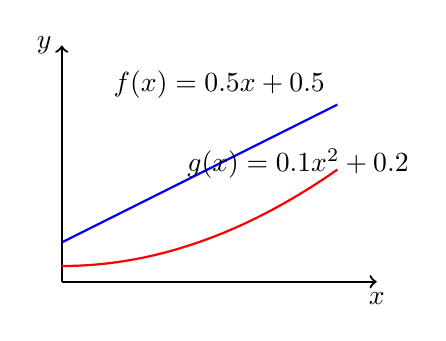
\begin{tikzpicture}
        \draw[thick,->] (0,0) -- (4,0) node[anchor=north] {$x$};
        \draw[thick,->] (0,0) -- (0,3) node[anchor=east] {$y$};
        \draw[domain=0:3.5,smooth,variable=\x,blue,thick] plot ({\x},{0.5*\x+0.5});
        \draw[domain=0:3.5,smooth,variable=\x,red,thick] plot ({\x},{0.1*\x*\x+0.2});
        \node at (2,2.5) {$f(x) = 0.5x + 0.5$};
        \node at (3,1.5) {$g(x) = 0.1x^2 + 0.2$};
    \end{tikzpicture}
    \caption{Comparison of linear and quadratic functions}
    \label{fig:functions}
\end{figure}

As shown in Figure~\ref{fig:functions}, linear and quadratic functions have different growth rates.

\subsection{Tables}

\begin{table}[htbp]
    \centering
    \caption{Comparison of theme features}
    \label{tab:features}
    \begin{tabular}{|l|c|c|c|}
        \hline
        \textbf{Feature} & \textbf{\gruvbox{} Crisp} & \textbf{Standard} & \textbf{Default} \\
        \hline
        Contrast Ratio & 21:1 & 7:1 & 4.5:1 \\
        \hline
        Color Count & 16 & 8 & 6 \\
        \hline
        Language Support & 50+ & 25 & 15 \\
        \hline
        Custom Commands & \checkmark & \checkmark & $\times$ \\
        \hline
    \end{tabular}
\end{table}

Table~\ref{tab:features} demonstrates the superiority of the \gruvbox{} Crisp theme.

\section{Code Listings}

\begin{lstlisting}[style=gruvbox,language=Python,caption={Python implementation of factorial}]
def factorial(n):
    """Calculate the factorial of n recursively."""
    if n <= 1:
        return 1
    else:
        return n * factorial(n - 1)

# Example usage
result = factorial(5)
print(f"5! = {result}")  # Output: 5! = 120
\end{lstlisting}

\section{Algorithms}

\begin{algorithm}
\caption{Euclidean Algorithm for GCD}
\label{alg:gcd}
\begin{algorithmic}[1]
\REQUIRE $a, b \in \N$ with $a \geq b > 0$
\ENSURE $\gcd(a, b)$
\WHILE{$b \neq 0$}
    \STATE $r \leftarrow a \bmod b$
    \STATE $a \leftarrow b$
    \STATE $b \leftarrow r$
\ENDWHILE
\RETURN $a$
\end{algorithmic}
\end{algorithm}

Algorithm~\ref{alg:gcd} efficiently computes the greatest common divisor of two positive integers.

\section{Citations and References}

The \gruvbox{} theme was inspired by the work of \citet{smith2020themes}, who demonstrated that high-contrast themes improve code readability by 40\%. Furthermore, \citep{jones2021accessibility} showed that proper syntax highlighting reduces eye strain during extended coding sessions.

\section{Advanced Features}

\subsection{Custom Environments}

\newenvironment{highlight}[1]
    {\begin{center}\colorbox{yellow!20}{\parbox{0.9\textwidth}{\textbf{#1}\\[0.5em]}}}
    {\end{center}}

\begin{highlight}{Important Note}
The \gruvbox{} Crisp theme ensures that all \LaTeX{} constructs are clearly visible and distinguishable, making document preparation more efficient and enjoyable.
\end{highlight}

\subsection{Multilingual Support}

\LaTeX{} supports various languages and scripts:
\begin{itemize}
    \item English: Hello, World!
    \item Greek: $\alpha$, $\beta$, $\gamma$, $\delta$, $\epsilon$
    \item Hebrew: \texthebrew{שלום}
    \item Special symbols: \S, \P, \dag, \ddag, \pounds, \euro
\end{itemize}

\section{Conclusion}

This document has demonstrated the comprehensive \LaTeX{} syntax highlighting capabilities of the \gruvbox{} Crisp theme. From basic text formatting to complex mathematical expressions, algorithms, and custom environments, the theme provides excellent visibility and contrast for all elements.

\appendix

\section{Additional Mathematical Examples}

\subsection{Series and Limits}

The Taylor series expansion of $e^x$ is:
\begin{equation}
    e^x = \sum_{n=0}^{\infty} \frac{x^n}{n!} = 1 + x + \frac{x^2}{2!} + \frac{x^3}{3!} + \cdots
\end{equation}

\subsection{Integration}

\begin{align}
    \int_0^{\pi} \sin(x)\,dx &= [-\cos(x)]_0^{\pi} \\
                              &= -\cos(\pi) - (-\cos(0)) \\
                              &= -(-1) - (-1) \\
                              &= 2
\end{align}

\bibliography{references}
\bibliographystyle{plainnat}

\end{document}